\documentclass[11pt,english,german]{report}

% Package import, Document Settings
\usepackage[a4paper,inner=3.5cm,outer=2.5cm]{geometry}
\usepackage[english,ngerman]{babel}
\usepackage[utf8]{inputenc}

% Packages
\usepackage[hyphens]{url}
\usepackage{caption}
\usepackage{latexsym}
\usepackage[T1]{fontenc}
\usepackage{graphicx}
\usepackage{hyperref}
\usepackage{tabularx}
\usepackage{etoolbox}
\usepackage{fancyhdr}
\usepackage{amsthm}
\usepackage{mathtools}
\usepackage[toc, acronym]{glossaries}
\usepackage{lastpage}
\usepackage{float}
\usepackage{makecell}
\usepackage{ltablex}
\keepXColumns
\usepackage{listings}
\usepackage{csquotes}
\usepackage{subcaption}
\usepackage{glossaries}
\usepackage{pdfpages}
\usepackage{fancyhdr}

\usepackage[
backend=biber,
style=alphabetic,
sorting=ynt
]{biblatex}
\addbibresource{datenbanken/references.bib}

\usepackage{titlesec}
\assignpagestyle{\chapter}{fancy}

\pagestyle{fancy}
\fancyhf{}
\rhead{\thepage}
\lhead{LIDAR Einbindung für den Robocup, \the\year}

\renewcommand\labelitemi{--}
\newcommand{\source}[1]{\caption*{Quelle: {#1}} }
\renewcommand{\chaptermark}[1]{\markboth{\MakeUppercase{#1}}{}}

\hypersetup{pdfborder = 0 0 0}


\definecolor{mygreen}{rgb}{0,0.6,0}
\definecolor{mygray}{rgb}{0.5,0.5,0.5}
\definecolor{mymauve}{rgb}{0.58,0,0.82}

\lstset{
	language=Java,
	numbers=left,
	columns=fullflexible,
	aboveskip=5pt,
	belowskip=10pt,
	basicstyle=\small\ttfamily,
	backgroundcolor=\color{black!5},
	commentstyle=\color{darkgreen},
	keywordstyle=\color{blue},
	stringstyle=\color{gray},
	showspaces=false,
	showstringspaces=false,
	showtabs=false,
	xleftmargin=16pt,
	xrightmargin=0pt,
	framesep=5pt,
	framerule=3pt,
	frame=leftline,
	rulecolor=\color{green},
	tabsize=2,
	breaklines=true,
	breakatwhitespace=true,
	prebreak={\mbox{$\hookleftarrow$}}
}

% Glossary
\makeglossaries

\setcounter{secnumdepth}{2}
\setcounter{tocdepth}{1}

\begin{document}
\newcommand{\titel}		{LIDAR Einbindung für den Robocup}
\newcommand{\versionnumber}	{abcdef}
\newcommand{\versiondate}	{\today}
\newcommand{\datum}		{\today}
\newcommand{\studiengang}	{Informatik, berufsbegleitend}
\newcommand{\autor}		{Marco Kilchhofer}
\newcommand{\betreuer}		{Dr. Reto Koenig, \acrshort{bfh}}
\newcommand{\auftraggeber}	{Alain Rohr, \acrshort{hftm} / Dr. Reto Koenig, \acrshort{bfh}}
\newcommand{\experte}		{Dr. Joachim Wolfgang Kaltz}


% Titelseite
\begin{titlepage}
\pagenumbering{Alph}
\begin{center}


\includegraphics[width=0.08\textwidth]{img/logo/bfh_logo.png}

Berner Fachhochschule | Haute école spécialisée bernoise | Bern University of Applied Sciences
\vspace{20mm}

\newcommand{\HRule}{\rule{\linewidth}{0.3mm}}
\HRule \\[0.4cm]
{\huge \titel}\\[0.3cm]
{\huge \bfseries  }
\HRule \\[2cm]


% Author und Dozent
\vfill
\end{center}
\begin{tabular}{ll}
	Studiengang:  & \studiengang 	\\
	Autor:        & \autor 		\\
	Betreuer:     & \betreuer	\\
	Auftraggeber: & \auftraggeber	\\
	Experte:      & \experte	\\
	Datum:        & \datum		\\
\end{tabular}

\end{titlepage}

\pagenumbering{Roman}

% Vorspann
\chapter*{Management Summary}
Die Höhere Fachschule für Technik Mittelland (HFTM) nimmt seit einigen Jahren mit dem Team ,,Solidus'' am internationalen RoboCup in der ,,Logistics League'' mit Erfolg teil. In der ,,Logistics League'' geht es darum, mit selber entwickelten Roboter in einer Produktionsanlage (Smart Factory) die Zwischenschritte - also die Logistik - zu automatisieren. Der Roboter bekommt beispielsweise den Auftrag aus dem Lager zur Anlage 1 Material zu bringen, oder von Anlage 2 die produzierten Teile abzuholen und ins Lager oder zu einer weiteren Produktionsanlage zu bringen. Die Roboter-Software ist mittlerweile relativ ausgereift für den aktuellen Cup. Das Team besteht jedes Jahr aus neuen Studenten die keinen vertieften Hintergrund in der Softwareentwicklung haben. Sie übernehmen die bestehende Code-Base vom vorherigen Team und müssen diese an die neuen Gegebenheiten anpassen und erweitern. Die historisch gewachsene, monolithische Architektur der Software wirkt diesen Anforderungen aber entgegen.

Das Ziel ist es, eine Softwarearchitektur und ein Entwicklungsvorgehen zu entwerfen, welche die Anforderungen an kurze Einarbeitungszeit und Flexibilität erfüllt. Fordert die geringere Effizienz der Umsetzung zwar mehr Ressourcen auf der Zielplattform, steigert sie dafür aber die Effizienz bei der Entwicklung.

In einer zeitgemässen Tool-Chain für die Entwicklung und einer Architektur basierend auf Microservices wurde die Anbindung eines Sensors (LiDAR) realisiert. Die einzelnen Schritte wurden so dokumentiert, dass sie in Schulungsunterlagen Verwendung finden können. So kann sichergestellt werden, dass zukünftige Entwicklungen voneinander abgekapselt in eigenständigen Microservices stattfinden können und somit keine direkte Abhängigkeit untereinander aufweisen. Die Kopplung und Datenkonversion der einzelnen Services wird mit Hilfe von domänenspezifischen Verbindern (Servants) realisiert.

Die exemplarische Entwicklung aus der Umsetzung zeigt, wie man künftig an der HFTM die Optimierung und Weiterentwicklung der Software angehen könnte. Das resultierende Dokument zu dieser Arbeit wurde so erfasst, dass es den zukünftigen HFTM-Studenten als Leitfaden dienen kann. Die Ausgangslage und die Umsetzung erlauben einen fliessenden Übergang in die neue Architektur.

% Inhaltsverzeichnis
\tableofcontents

% Content
\chapter{Einleitung}
\pagenumbering{arabic}
Die Studenten der Höheren Fachschule für Technik Mittelland (\acrshort{hftm}) aus der Studienrichtung Systemtechnik nehmen seit einigen Jahren am internationalen RoboCup teil. Dazu kommt ein Roboter mit selbst entwickelter Hard- und Software zum Einsatz. Unter dem Team-Namen ,,Solidus'' spielen die Studenten am RoboCup bereits an der Spitze mit (2. und 3. Platz). Das Team besteht nebst dem Dozenten Alain Rohr jedes Jahr aus neuen Studenten die keinen vertieften Hintergrund in der Softwareentwicklung haben. Sie übernehmen die bestehende Code-Base vom vorherigen Team und müssen diese an die neuen Gegebenheiten anpassen und erweitern. Beispielsweise ändert sich jährlich die Umgebung (Lichtverhältnisse, etc.), die Cup-Regeln und es müssen neue Sensoren oder Aktoren integriert werden. Die historisch gewachsene, monolithische Architektur der Software wirkt diesen Anforderungen aber entgegen.
Sie baten die BFH um Hilfe beim Software-Engineering. Es geht in dieser Arbeit also darum, ein Design für die Roboter-Software zu entwerfen, so dass die Studenten unabhängig voneinander entwickeln können.
\section{RoboCup}
Der RoboCup ist ein Wettbewerb, der seit 1997 jährlich ausgetragen wird \cite{wikipedia-robocup}. Ursprünglich ging es hauptsächlich darum, Roboter zu entwickeln, die gegeneinander Fussball spielen. Das langfristige Ziel dieses Wettbewerbs \cite{wikipedia-roboterfussball}: 
\begin{formal}
im Jahr 2050 den menschlichen Weltmeister in einem gewöhnlichen Fussballspiel zu schlagen
\end{formal}
Es kommen jedoch immer neue Ligen dazu. Der aktuelle Stand an Ligen für den RoboCup 2018 ist in Screenshot aus Abbildung \ref{fig:robocup_ligen} ersichtlich.
\begin{figure}[H]
	\centering
	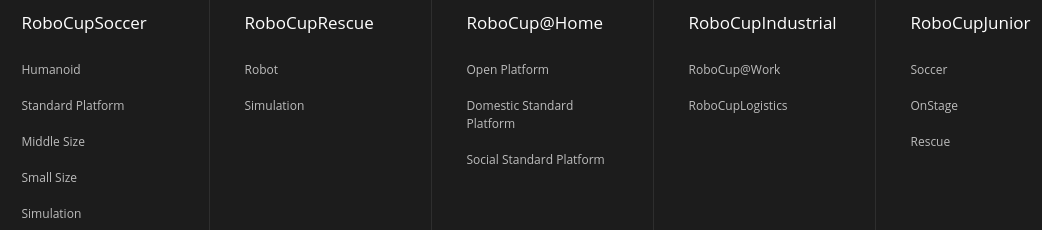
\includegraphics[width=\textwidth]{img/robocup-ligen.png}
	\caption{RoboCup Ligen, Screenshot von \cite{www.robocup.org}}
	\label{fig:robocup_ligen}
\end{figure} 
So gibt es beispielsweise in der Disziplin ,,RoboCupSoccer'' die Liga ,,Humanoid''. Die Roboter aus dieser Liga sind auch in den Medien hierzulande sehr bekannt. Im Bild \ref{fig:robocup_fussball} ist ein solcher Humanoid beim Fussballspielen am RoboCup zu sehen.
\begin{figure}[H]
	\centering
	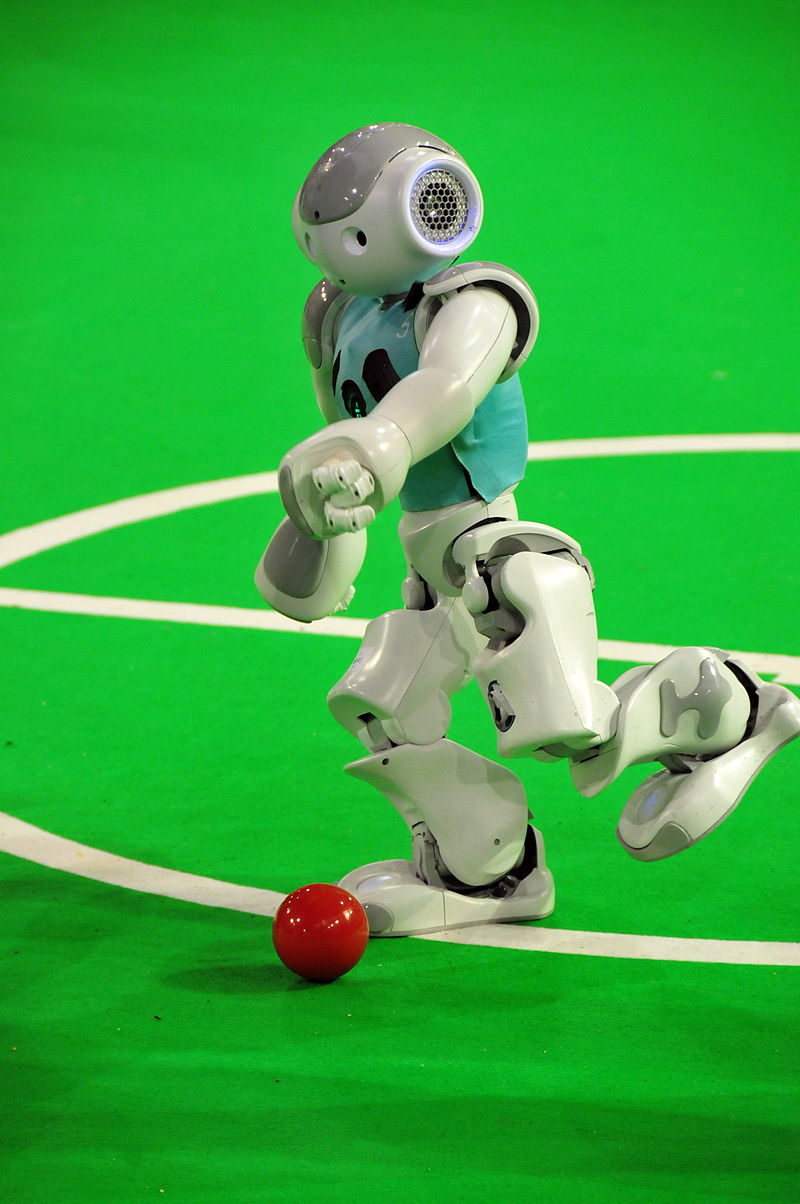
\includegraphics[width=0.2\textwidth]{img/robocup-humanoid.jpg}
	\caption{Roboter beim Fussball spielen. Quelle: Ralf Roletschek / roletschek.at \cite{robocup2013}}
	\label{fig:robocup_fussball}
\end{figure}
\subsection{RoboCupLogistics}
Seit 2012 gibt es am RoboCup die Liga ,,Logistics'', die wie folgt spezifiziert ist \cite{wikipedia-robocup}:
\begin{formal}
	Ziel dieser Liga ist die Entwicklung von autonom agierender Roboter zur Steuerung des Material- und Informationsflusses in industriellen Produktionsanlagen.
\end{formal}
Es spielen zwei Teams gegeneinander mit jeweils 3 Robotern. Auf dem  Spielfeld (Abbildung \ref{fig:robocup_spielfeld}) sind pro Team zufällig sieben Maschinen  aufgestellt. Diese müssen von den Robotern erkundet werden. Dafür hat jede Maschine vorne und hinten einen eindeutigen 2D-Code aufgedruckt, dem so genannten AR Tag (Prinzip ähnlich einem QR-Code). Jede Maschine repräsentiert eine Station in einer Produktionsanlage (einer ,,smart factory''). An jeder Station können Gegenstände zugebracht und auf der gegenüberliegenden Seite entnommen werden. Kontrolliert, überwacht und bewertet wird das Spiel von der ,,Referee Box''. Von ihr werden die 'Active orders' (Bestellungen) verwaltet und publiziert, die die Roboter auf dem Spielfeld umsetzen müssen. Sie koordiniert auch die Maschinen auf dem Spielfeld, zu denen die Roboter fahren müssen, um Gegenstände zu bringen und abzuholen.
\begin{figure}[H]
	\centering
	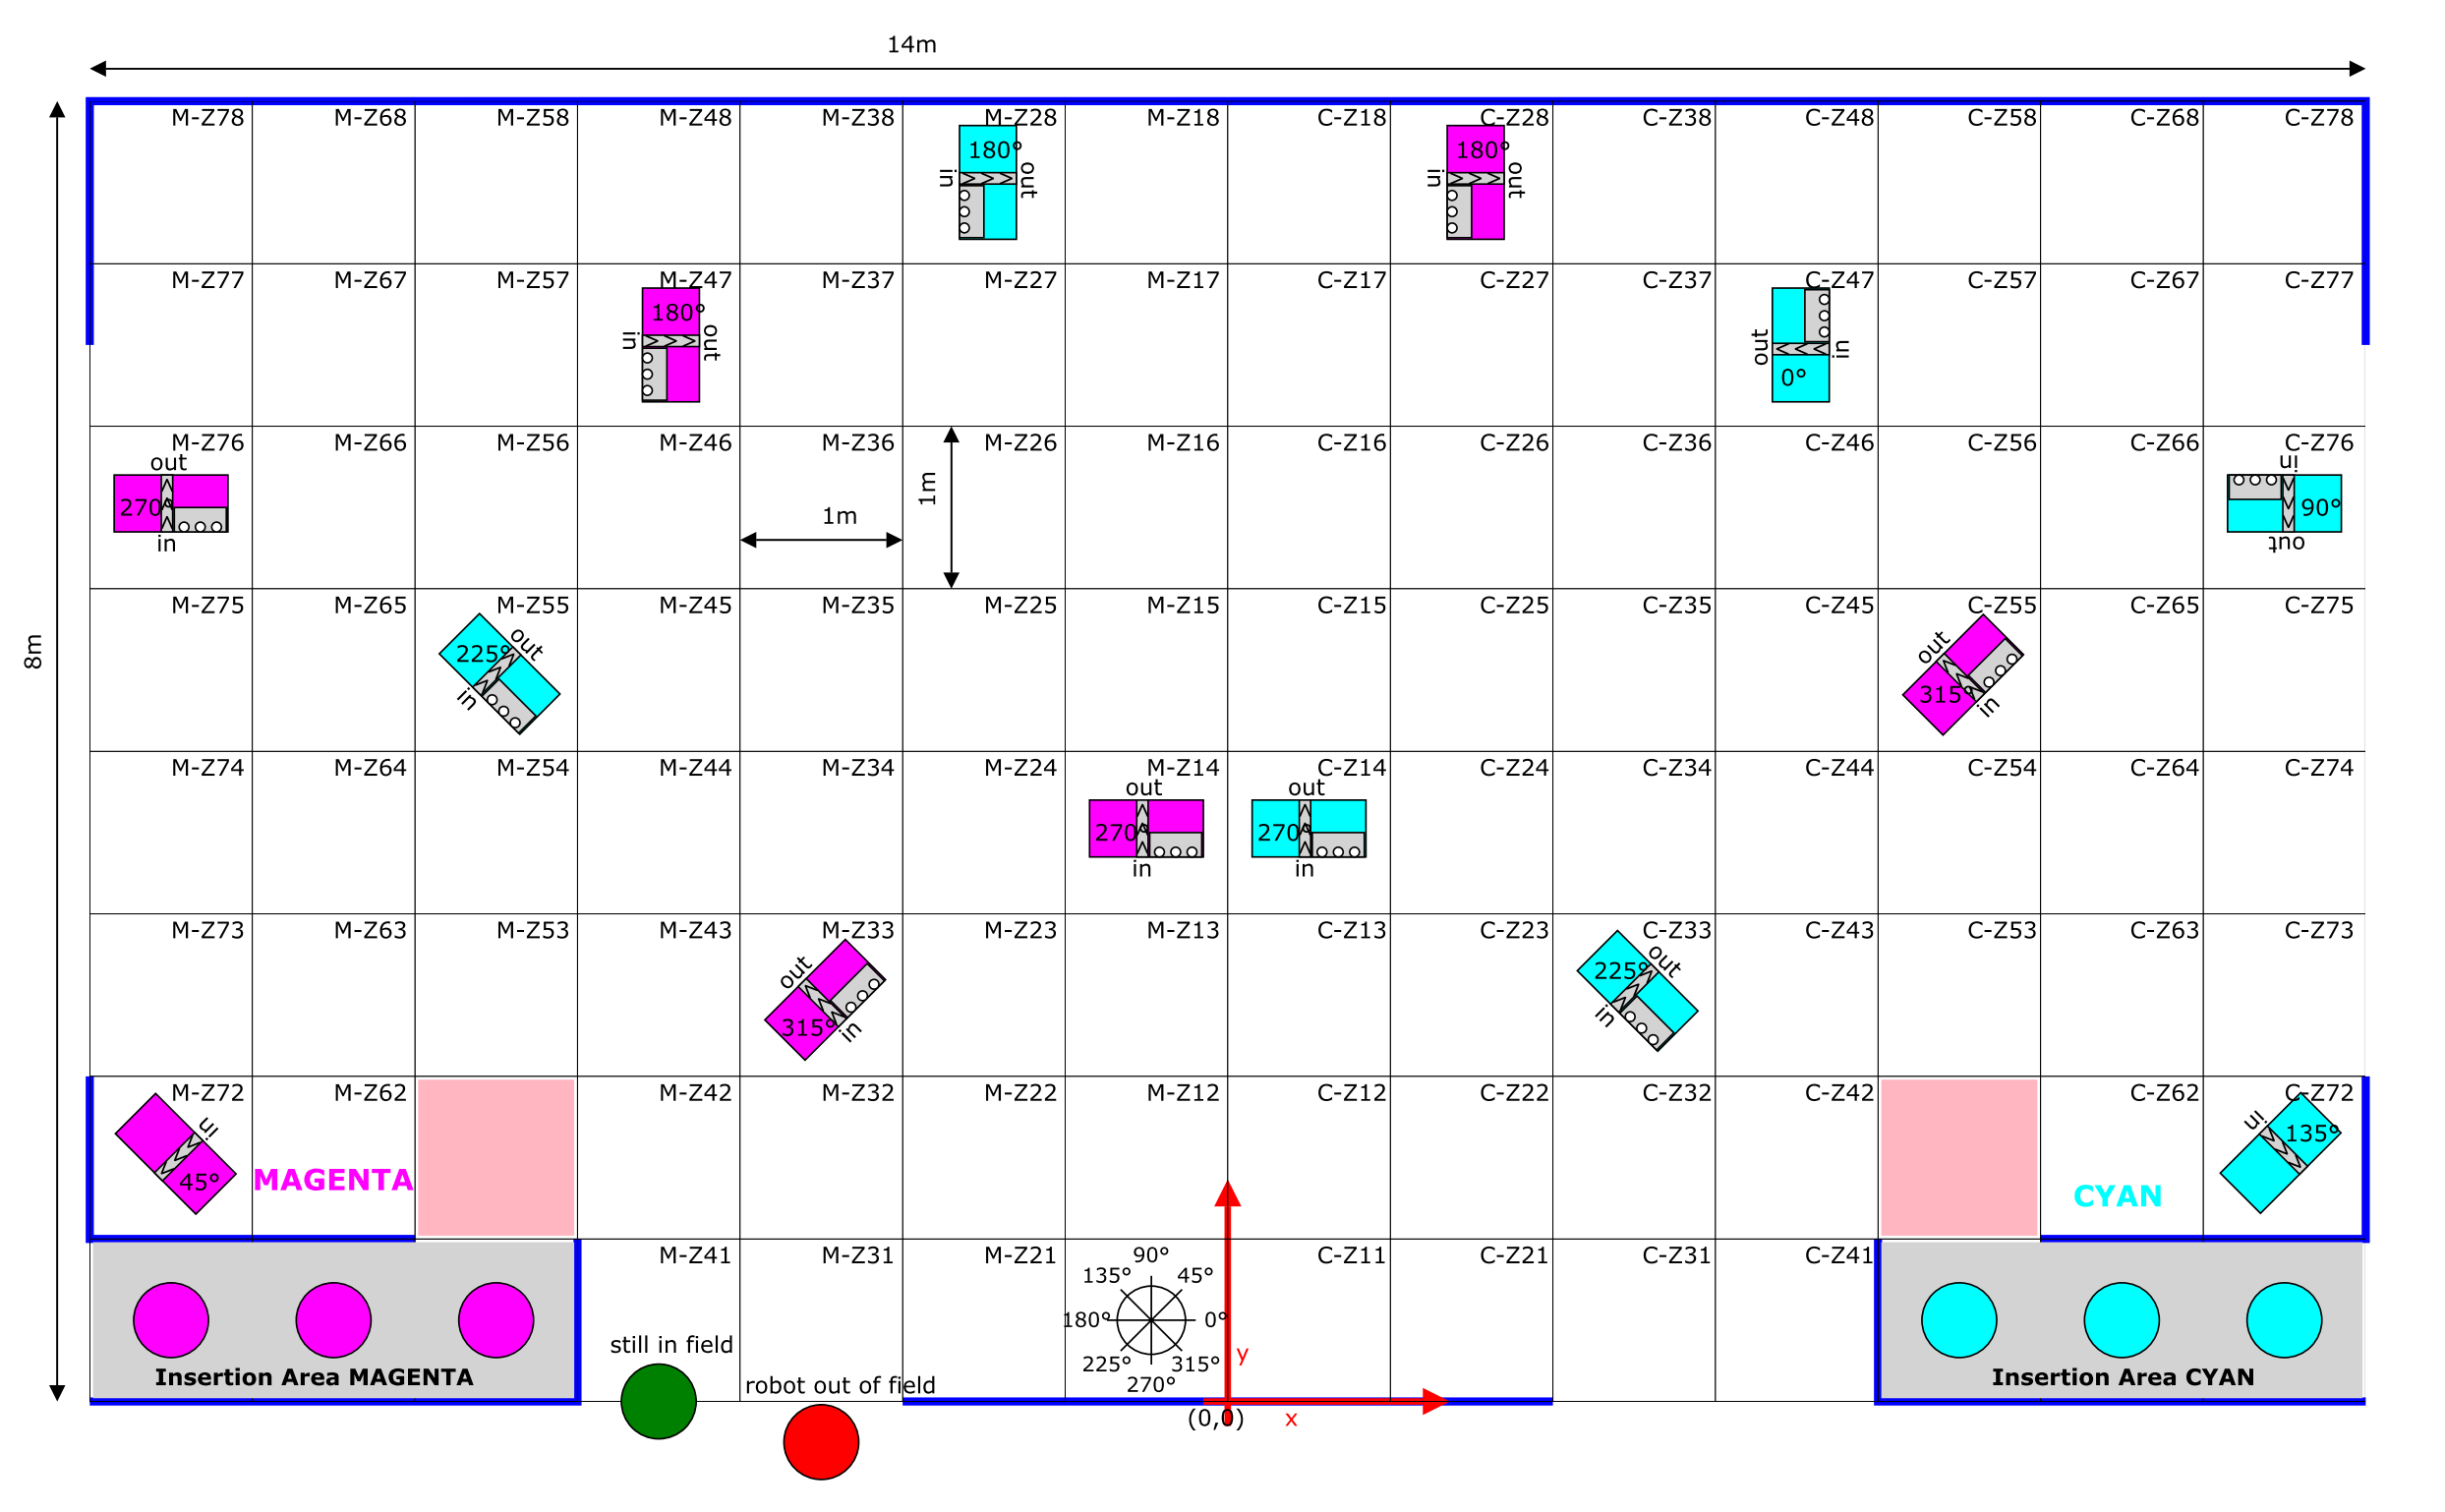
\includegraphics[width=0.75\textwidth]{img/robocup-spielfeld-2d.png}
	\caption{Spielfeld mit möglicher Aufstellung der Maschinen: Quelle: robotics-erlangen.de \cite{robotics-erlangen.de}}
	\label{fig:robocup_spielfeld}
\end{figure}

Die verwendeten Roboter in dieser Liga basieren auf der ,,Robotino''-Plattform  von Festo (Abbildung \ref{fig:robotino}), die den Wettbewerb auch mit den Maschinen und anderem sponsern. Auf dieser Roboterplattform können verschiedene Sensoren, Aktoren und Computer-Systeme angebaut werden.
\begin{figure}[H]
	\centering
	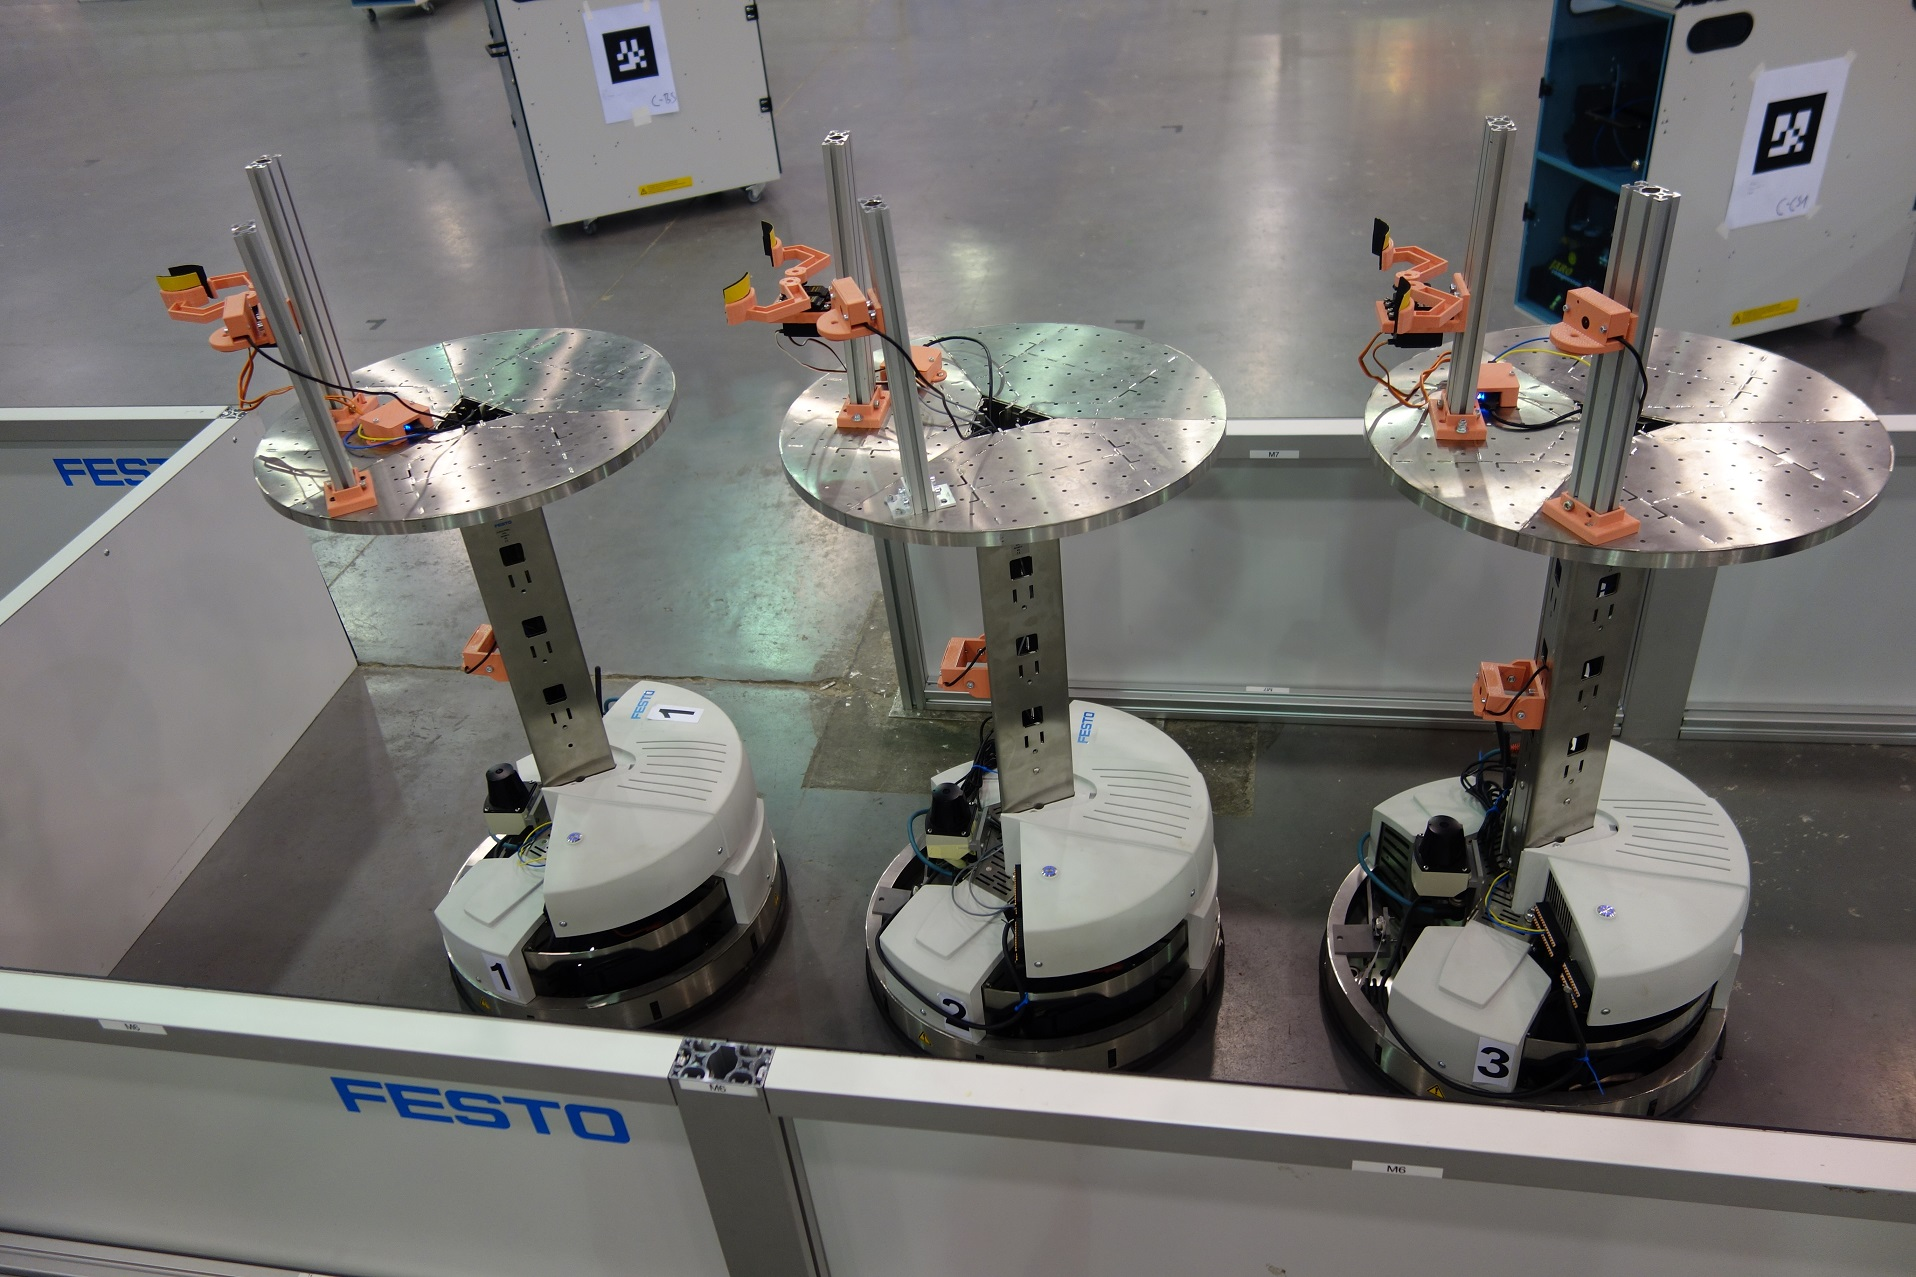
\includegraphics[width=0.5\textwidth]{img/robotino_v3.jpg}
	\caption{Robotino v3 für die Logistics League\cite{robotino}}
	\label{fig:robotino}
\end{figure}



\section{\acrshort{lidar}}
Diese Arbeit zeigt anhand eines \acrshort{lidar}-Sensors, wie ein mögliches Software-Design für den Roboter aussehen kann. Doch was ist \acrshort{lidar}?
\begin{formal}
	Lidar ist eine dem Radar verwandte Methode zur optischen Abstands- und Geschwindigkeitsmessung sowie zur Fernmessung atmosphärischer Parameter. Statt der Radiowellen wie beim Radar werden Laserstrahlen verwendet. \cite{wikipedia-lidar}
\end{formal}
Meistens versteht man unter em Begriff \acrshort{lidar} gleich einen Sensor, wie er auch in dieser Arbeit verwendet wird. Sie messen nicht nur in eine Richtung, sondern fast die ganze Umgebung um den Sensor herum. Der in dieser Arbeit verwendete TiM55x kann 270° der Umgebung ausmessen. Solche Sensoren kommen beispielsweise bei Fahrzeugen mit Autopilot (Bsp. Tesla) zum Einsatz um die Hindernisse in der Umgebung zu erkennen. Im Prinzip funktionieren solche Sensoren ähnlich wie eine Radar-Bodenstation in der Luftfahrt: Über ein drehendes Element (bei \acrshort{lidar} einen Spiegel) werden kontinuierlich Laserstrahl-Impulse ausgesendet. Wenn sich ein Objekt in der Nähe des Sensors befindet, trifft dieser Laserstrahl das Objekt und ein Teil davon wird reflektiert. Die Reflexion detektiert der Sensor und errechnet daraus die resultierende Distanz zum Objekt.
\begin{figure}[H]
	\centering
	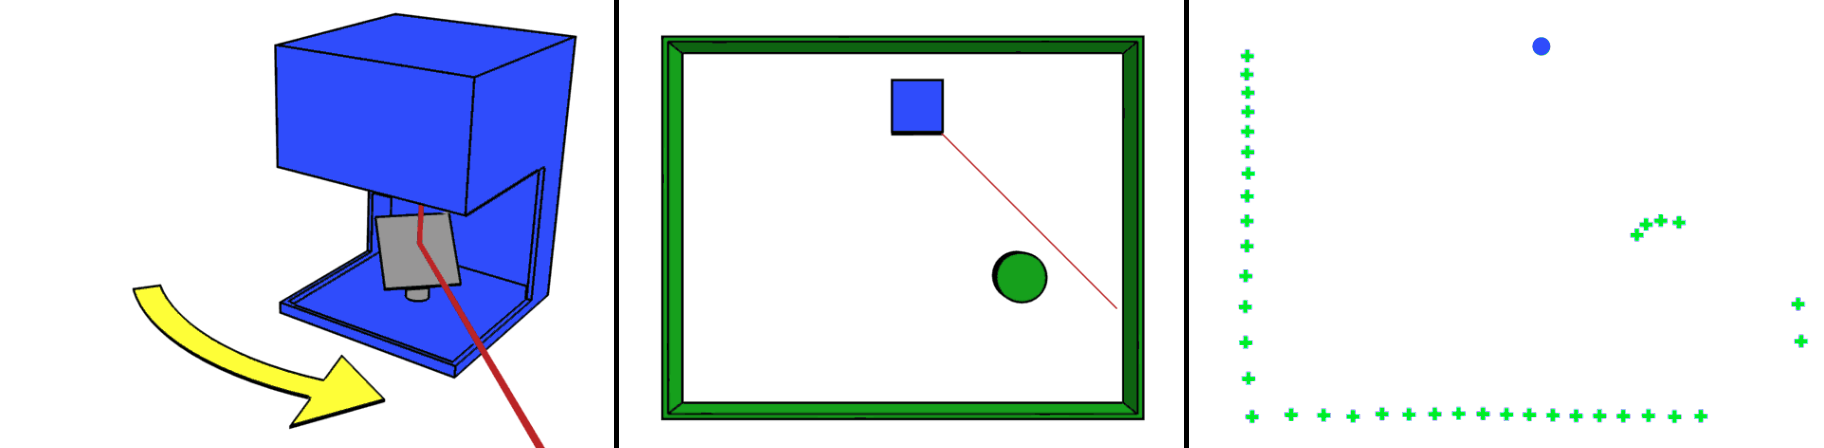
\includegraphics[width=0.7\textwidth]{img/lidar-principle.png}
	\caption{Prinzip 2D-Abtastung mit Lidar \cite{wikipedia-lidar}}
	\label{fig:lidar-principle}
\end{figure}


\subsection{SICK TiM55x}
\label{chap:tim55x}
Die Funktionsweise des verwendeten Sensors ist im Datenblatt vom Hersteller SICK wie folgt beschrieben \cite{tim55x-techinfo}:
\begin{formal}
Der TiM5xx sendet mit einer Laserdiode gepulste Laserstrahlen aus. Trifft ein solcher Laserpuls auf ein Objekt oder eine Person, wird er an dessen Oberfläche reflektiert. Die Reflexion wird im Empfänger des TiM5xx von einer Fotodiode registriert. Der TiM5xx nutzt die SICK-eigene HDDM-Technologie (High Definition Distance Measurement). Bei diesem Messverfahren wird ein Messwert durch die Mittelwertbildung mehrerer Einzelpulse gebildet. Aus der Laufzeit, die das Licht von der Aussendung des Strahls bis zum Empfang der Reflexion benötigt, berechnet der TiM5xx die Entfernung zum Objekt. Dieses Prinzip der ,,Pulslaufzeitmessung'' wird in ähnlicher Form von Radarsystemen benutzt.

Mit einem rotierenden Spiegel lenkt der TiM5xx die ausgesendeten Laserstrahlen ab und tastet damit die Umgebung radial ab. Die Messungen werden intern von einem Winkelkodierer in regelmässigen Winkelschritten ausgelöst. Eine komplette Rotation stellt einen Messvorgang (Scan) dar. Der TiM5xx arbeitet mit einer Scanfrequenz von 15 Hz, d. h. er durchläuft 15 Messvorgänge pro Sekunde und stellt die Messergebnisse fortlaufend in Echtzeit über die Ethernet-Schnittstelle zur Verfügung.
\end{formal}

Wir erhalten also von diesem Sensor 15 Mal Sekunde eine komplette Messung mit 270 Distanzen und der dazugehörigen Genauigkeit. Diese Messwerte sind wie im Datenblatt beschrieben wie folgt zu verstehen: Der erste Messwert erhalten wir bei -45° und der letzte bei 225° (siehe dazu Abbildung \ref{fig:lidar}). Der TiM55x-Sensor ist an der Robotino-Plattform so verbaut, dass 90° vorne entspricht. Weshalb der Hersteller negative Werte im Koordinatensystem verwendet hinterfragen wir nicht weiter. Die zu entwickelnde Software soll also genau diesen Winkel-Bereich zur Verfügung stellen - so steht er auch im Datenblatt.
\begin{figure}[H]
	\centering
	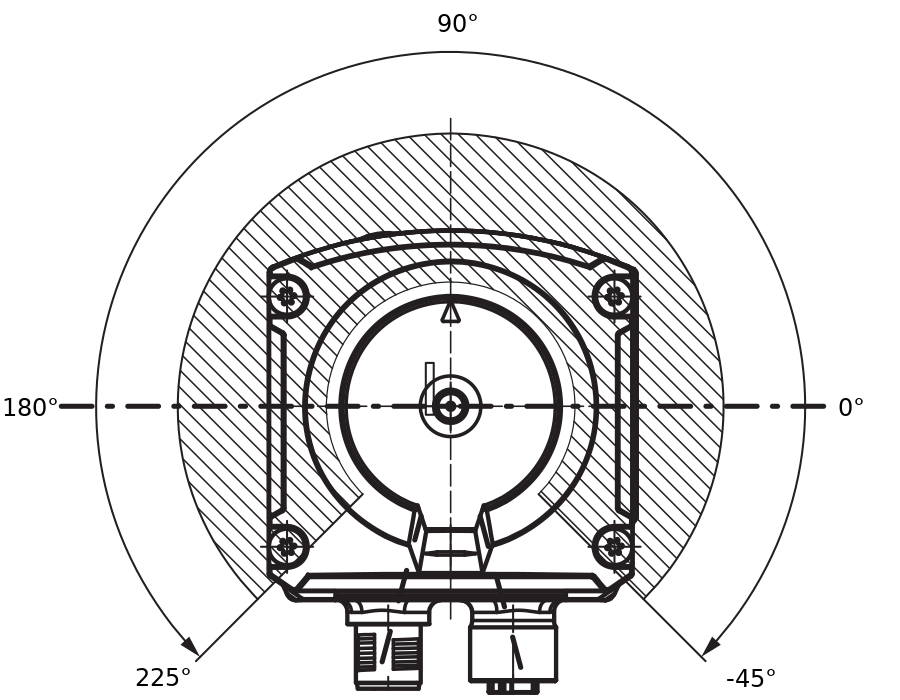
\includegraphics[width=0.5\textwidth]{img/lidar-coordinate.png}
	\caption{\acrshort{lidar}: Draufsicht / Koordinatensystem}
	\label{fig:lidar}
\end{figure}

\chapter{Grundlagen}
\label{chap:voraussetzungen}
Dieses Kapitel soll oberflächlich einige Dinge erklären, die für diese Arbeit vorausgesetzt werden.
\section{Apache Maven}
\label{chap:maven}
Maven ist ein Tool um den Build-Prozess von Software zu unterstützen. Es bietet beispielsweise Unterstützung fürs Managen der Abhängigkeiten, fürs Testing und zur Paketierung. Die zu entwickelnden Services aus Kapitel \ref{chap:beispielimplementation} verwenden Maven vor allem für das Dependency-Management. Konkret ist Maven in diesem Projekt für folgendes zuständig:
\begin{itemize}
	\item
	Libraries müssen nicht manuell heruntergeladen und ins Projekt aufgenommen werden.
	\item
	Versionen der Libraries sind zentral definiert. Ein Upgrade einer Library auf eine neue Version lässt sich somit an einem Ort erledigen.
	\item
	Paketierung der Services/Applikationen als Jar-Datei.
\end{itemize}
Um Maven zu verwendet erstellt man in der verwendeten Entwicklungsumgebung (\acrshort{ide}) ein 'Maven-Projekt'. Zentral in einem Maven-Projekt ist die Datei \texttt{pom.xml} (\acrshort{pom} steht für \acrlong{pom}). Sie definiert wie oben erläutert die Umgebung für das Java-Projekt.

\subsection{Dependencies}
Maven verwendet so genannte Repositores um Libraries anzuziehen. Repositories können lokal oder remote sein. Dependencies/Libraries sucht man beispielsweise auf \texttt{mvnrepository.com}. Alle Libaries in diesem Repository kennt Maven automatisch und kann diese herunterladen. Heruntergeladen werden die Libraries (als Jar paketiert) in das lokale Repository, also in den Ordner \texttt{.m2} im Home-Verzeichnis des ausführenden Benutzers. In dieser Arbeit ist das also \path{/home/mkilchhofer/.m2/repository} (Fedora Linux) und unter Windows wird das in \path{C:\Users\mkilchhofer\.m2\repository} sein.

Als kurzes Beispiel hier eine Demonstration zur Einbindung von Log4j2.
\begin{enumerate}
	\item Auf mvnrepository nach ,,Log4j Core'' suchen.
	\item Version auswählen (hier zum Beispiel ,,2.11.0'')
	\item XML-Struktur (Abbildung \ref{fig:mvnrepository-example}) im \texttt{pom.xml} in den Sub-Baum \texttt{<dependencies>} einfügen (Listing \ref{lst:maven-example-simple})
\end{enumerate}

\begin{figure}[H]
	\centering
	\includegraphics[width=0.7\textwidth]{img/voraussetzung/mvnrepository-example.png}
	\caption{Code zum kopieren von \texttt{mvnrepository.com}}
	\label{fig:mvnrepository-example}
\end{figure}

\begin{lstlisting}[language=XML, caption={Simples Beispiel wie ein pom.xml aussieht},label={lst:maven-example-simple}]
<?xml version="1.0" encoding="UTF-8"?>
<project /* ... (generiert die IDE) ... */>
	<modelVersion>4.0.0</modelVersion>
	<artifactId>lidar-hardware-service</artifactId>
	<groupId>info.kilchhofer.bfh</groupId>
	<version>1.1-SNAPSHOT</version>
	<packaging>jar</packaging>

	<dependencies>
		<dependency>
			<groupId>org.apache.logging.log4j</groupId>
			<artifactId>log4j-core</artifactId>
			<version>2.11.0</version>
		</dependency>
	</dependencies>
</project>
\end{lstlisting}
Maven übernimmt dann über die \acrshort{ide} den Rest und lädt das Jar und nötigenfalls die Sources an die erforderlichen Orte herunter.
\subsection{Maven Lifecycle}
In jeder aktuellen \acrshort{ide} ist Maven sehr gut eingebunden. So taucht bei einem maven-managed Projekt in der \acrshort{ide} \textit{\Gls{intellij}} folgende Komponente an der rechten Seite auf:
\begin{figure}[H]
	\centering
	\includegraphics[scale=0.5]{img/voraussetzung/maven-lifecycle-ide2.png}
	\caption{Maven Lifecycle in der \acrshort{ide}}
	\label{fig:maven-ide}
\end{figure}
Durch das Auswählen der jeweiligen Lifecycle-Phase mit anschliessendem Drücken auf den Play-Knopf wird der entsprechende Task ausgeführt. Was die einzelnen Phasen (Tasks) genau machen ist folgender Tabelle \ref{tab:mavenLifecycle} zu entnehmen.

\begin{table}[H]
	\centering
	\begin{tabular}{lp{13cm}} \toprule
		\textbf{Lifecycle} & \textbf{Beschreibung}\\ \midrule
		\texttt{clean}     & Alle generierten Objekte (namentlich 'Artefakte') und das Verzeichnis '\path{target}' werden gelöscht.\\ \midrule
		\texttt{validate}  & Validieren ob alle Projekt-Infos vorhanden und korrekt sind (vor allem pom.xml prüfen).\\ \midrule
		\texttt{compile}   & Kompiliert den Source-Code des Projekts. Syntax-Fehler im Verzeichnis '\path{src/main/..}' lassen diese Phase Fehlschlagen. Die Tests aus dem Verzeichnis '\path{src/test/..}' werden in dieser Phase noch nicht berücksichtigt. Syntax-Fehler in den Unit-Tests beeinflussen das erfolgreiche Abschliessen dieser Phase nicht.\\ \midrule
		\texttt{test}	   & Führt die Tests gegen den kompilierten Source-Code aus. Diese Tasks endet erfolgreich, wenn die Syntax aller Tests fehlerfrei sind und die Tests erfolgreich durchgeführt werden können.\\ \midrule
		\texttt{package}   & Paketiert den generierten Byte-Code in ein verteilbares Archiv (Bsp. Jar)\\ \midrule
		\texttt{verify}	   & Prüft die paketierten Datein mittels Integrations-Tests.\\ \midrule
		\texttt{install}   & Kopiert die paketierten Dateien in das lokale Maven Repository (\path(.m2)-Ordner), um diese als Abhängigkeit in anderen lokalen Projekten zu benutzen.\\ \midrule
		\texttt{site}      & Generiert eine Projekt-Website \\ \midrule
		\texttt{deploy}	   & Kopiert das generierte Artefakt in ein remote Maven Repository (gleich wie \texttt{install}, nur eben Remote.)				\\ \bottomrule
	\end{tabular}
	\caption{Basic Lifecycle-Phasen in Maven. Quelle: \href{https://maven.apache.org}{maven.apache.org} \cite{maven-build-lifecycle} }
	\label{tab:mavenLifecycle}
\end{table}



\section{Tests / Unit Tests}
Der zu entwickelnde Programmcode soll wie folgt automatisch auf zwei Stufen getestet werden:
\begin{itemize}
	\item Unit Tests (Klassen und Methoden)
	\item Integrationstests der verschiedenen Microservices
\end{itemize}
Die umgesetzten Tests verwenden JUnit als Framework.  Der Aufbau von JUnit Tests zeigt dieses kleine Beispiel:
\begin{lstlisting}[caption={Simples Beispiel wie JUnit funktioniert},label={lst:junit-example-simple}]
package info.kilchhofer.bfh.lidar.hardwareservice;

import org.junit.jupiter.api.Test;
import static org.junit.jupiter.api.Assertions.assertEquals;
import static org.junit.jupiter.api.Assertions.assertNotEquals;

public class SimpleTest {
	@Test
	@DisplayName("myInt durch 2 teilbar aber nicht durch 3")
	public void mySimpleTest(){
		int myInt = 1024;
		assertEquals(0, (myInt % 2));
		assertNotEquals(0, (myInt % 3));
	}
	
	@Test
	@DisplayName("Log2")
	public void mySimpleTest2(){
		int temp = (int) (Math.log(myInt) / Math.log(2));
		assertEquals(9, temp);
	}
}
\end{lstlisting}
Führt man diesen Test in der \acrshort{ide} \textit{\Gls{intellij}} aus, bekommt man folgenden Output:
\begin{figure}[H]
	\centering
	\includegraphics[width=0.7\textwidth]{img/voraussetzung/junit-example.png}
	\caption{JUnit Beispieldurchlauf}
	\label{fig:junit-example}
\end{figure}
Wie zu erwarten, schlägt der zweite Test fehl, weil der Logarithmus zur Basis 2 von 1024 natürlich 10 ist. Der Erwartungswert im Test ,,Log2'' ist aber 9.

Beispiele die sich auf den entwickelten Code beziehen gibt es im Abschnitt mit der Beispielimplementation (Kapitel \ref{chap:beispielimplementation}).

\section{Git}
Als \acrshort{vcs} setzen wir Git ein. Ins Git gehört jeglicher entwickelte Code, nicht aber Artefakte (gebuildeter Code) und IDE spezifische Einstellungen. Die entsprechenden Verzeichnisse müssen wir also in \path{.gitignore}-Datei aufnehmen.

\section{MQTT}
\label{sec:mqtt}
TODO - Stichworte: \acrshort{mqtt}, Broker, Client, publish, subscribe

\chapter{Software Design}
In diesem Kapitel wird ein mögliches Design für den Robocup erläutert.
\section{Einführung}
Bis anhin hat die \acrshort{hftm} mit dem Team Solidus am Robocup bereits an der Spitze mitgespielt. So fragt man sich vielleicht, wieso diese Arbeit überhaupt zu Stande kommt. Bis heute entwickelt man mit einem monolithischen Ansatz. Das Meiste ist eng miteinander verzahnt und die Software lässt sich schwer und mit viel Zeit weiterentwickeln. Der Roboter für den Wettbewerb wird gleichzeitig aber ständig komplexer und es müssen immer wieder neue Dinge (Bsp. Sensoren) integriert werden. Auch müssen sich die Schüler jedes Jahr durchgehend mit allen Schichten bzw. Teilen (von Hardware bis Business-Logik) neu befassen. In den nachfolgenden Abschnitten soll gezeigt werden, wie man die einzelnen Systeme des Roboters in Domänen (Positionierung, Fahr-Einheit, Greifsystem, etc.) unterteilt und dazwischen simple und nachhaltigere Schnittstellen realisieren kann.
Jede einzelne Komponente im System verwendet zum Austausch mit Anderen den Systemweiten Event-Bus, egal zu welcher Domain sie gehört.

\section{Monolith vs. Microservice}
Man hört es heute an jedem Enwickler-Event, liest es in verschiedenen Zeitschriften, egal ob für Entwickler oder System-Administratoren: der Weg zum Ziel sollen Microservices sein, sie sollen Monolithen ablösen. Viele kleine Services statt einen grossen, verzahnten und schwierig wartbaren Moloch.
In \cite{informatik-aktuell-microservices} findet sich ein passendes Statement zur monolithischen Applikation:
\begin{quote}
	Selbstverständlich startet keine Neuentwicklung als ,,grosser Monolith". Anfangs ist die Anwendung schlank, leicht zu erweitern und gut zu verstehen – die Architektur adressiert die Probleme, die das Team zu dieser Zeit hat. Im Laufe der Monate entsteht mehr und mehr Code. Es werden Schichten definiert, Abstraktionen gefunden, Module, Services und Frameworks eingeführt, um die wachsende Komplexität in den Griff zu bekommen.
	
	Bereits bei mittelgrossen Anwendungen (etwa eine Java-Anwendung mit mehr als 50.000 LOC\footnote{Lines of Code}) werden monolithische Architekturen langsam unangenehm. Das gilt vor allem für Anwendungen, die hohe Anforderungen an die Skalierbarkeit stellen. Aus der schlanken Neuentwicklung entwickelt sich das nächste Legacy-System, über das folgende Generationen von Entwicklern fluchen werden.
\end{quote}
Die Vorteile von Microservices sprechen für sich. Hier ein Auszug der wichtigsten Punke aus der selben Quelle\cite{informatik-aktuell-microservices}, die für den Roboter interessant sind:
\begin{itemize}
	\item
Aufgrund ihrer geringen Grösse benötigt man wenig Boiler-Plate Code und keine schwergewichtigen Frameworks.
	\item
Sie lassen sich unabhängig voneinander deployen. Continuous Delivery bzw. Deployment lässt sich damit sehr viel einfacher realisieren.
	\item
Die Architektur unterstützt die Arbeit in mehreren, unabhängigen Teams.
	\item
Es ist pro Service möglich, die jeweils „beste“ Programmiersprache zu wählen. Man kann ohne grosses Risiko auch mal eine neue Sprache, ein neues Framework oder ähnliches ausprobieren. Man sollte es dabei nur nicht übertreiben.
	\item
Da sie klein sind, lassen sie sich auch jederzeit mit vertretbarem Aufwand durch eine Neuentwicklung ablösen.
	\item
Microservices kommen der agilen Entwicklung entgegen. Ein neues Feature, von dessen Erfolg beim Kunden man noch nicht überzeugt ist, lässt sich nicht nur schnell entwickeln – es lässt sich auch schnell wieder wegwerfen.
\end{itemize}


\section{Architektur}
Im Kapitel \ref{sec:mqtt} wird beschrieben, dass auf dem Roboter bis jetzt bereits einiges über den Event-Bus \acrshort{mqtt} kommuniziert. Dies bildet auch die zentrale Komponente in der neuen Architektur. Es gäbe auch andere Event-Busse, die dafür verwendet werden könnte (Bsp. \acrshort{ros}). \acrshort{mqtt} ist beispielsweise durch die Verwendung in Heimautomationen bereits weit verbreitet und es gibt bereits Libraries für unterschiedliche Programmiersprachen und eine grosse Community dafür, aber vor allem kennen die Studenten der HFTM dies bereits. Es sollen Micro-Services entstehen, die nur genau eine Aufgabe erfüllen. Nämlich das hardware-spezifische Protokoll zwischen Hardware (hier \acrshort{lidar}) und der \acrshort{mqtt}-Welt zu adaptieren. \Glspl{service} kennen sich untereinander nicht, sie wissen nichts von der Existenz anderer \glspl{service}. Damit die einzelnen \Glspl{service} miteinander kommunizieren können, kommen so genannte \Glspl{servant} zum Einsatz. Diese kennen die Schnittstellen (\gls{contract}/\acrshort{api}) der zu bedienenden Services. Wir werden dieses Konzept in den nachfolgenden Kapitel am Beispiel des \acrshort{lidar} anschauen.

\begin{figure}[H]
	\centering
	\includegraphics[width=0.6\textwidth]{img/architecture/highlevel.png}
	\caption{Architektur in Domains}
	\label{fig:architecture_highlevel}
\end{figure}





\section{Aufbau eines Services, Begriffe}
Jeder Service im System soll sich an in diesem Abschnitt beschriebenen Grundsatz halten. Die Basis dazu liefert das ab dem sechsten Semester kennengelernte Muster mit Intent, Status und Event für die MQTT Topics. Die Java-Library ch.quantasy.mqtt.gateway\cite{ch.quantasy.mqtt.gateway} von Reto Koenig implementiert dies bereits so. Die \acrshort{mqtt}-Topics stellen das \acrshort{api} für den jeweiligen Service dar und liefert bzw. konsumiert eine Dokumentstruktur mit \acrshort{yaml}-Inhalt. Die nachfolgenden Teilabschnitte basieren demzufolge auf dem englischen README von Github\cite{ch.quantasy.mqtt.gateway}. In Abbildung \ref{fig:gatewayclient} ist ersichtlich welche Basis-Topics bzw. \acrshort{api}s in Richtung MQTT-Broker zur Verfügung stellt.

\begin{figure}[H]
	\centering
	\includegraphics[width=0.6\textwidth]{img/ch.quantasy.mqtt.gateway/MqttGatewayClient.png}
    \caption{GatewayClient, ch.quantasy.mqtt.gateway\cite{ch.quantasy.mqtt.gateway}}
    \label{fig:gatewayclient}
\end{figure}



\subsection{Unit}
Als \gls{unit} wir eine Instanz eines Services oder generell eines GatewayClients bezeichnet. Im Hardware-Service für den \acrshort{lidar}-Sensor wird pro konfigurierter Sensor eine Instanz des GatewayClients erstellt. Das sind also unterschiedliche Units.
\subsection{Intent}
Kann ein Service Befehle über die \acrshort{api} auf der Seite von \acrshort{mqtt} entgegennehmen, so werden diese über das Topic '\gls{intent}' dem Service mitgeteilt. Pro Service gibt es nur ein Intent-Topic.
\subsection{Status}
Mehrheitlich statische Informationen stellt ein Service unter dem Basis-Topic '\gls{status}' zur Verfügung. Unter diesem Topic kann eine beliebige Baumstruktur aufgebaut werden.
\subsection{Event}
TODO
\subsection{Description}
Im Topic '\gls{description}' beschreibt ein Service bzw. eine \acrshort{unit} beim Aufstarten bzw. beim Instanziieren des GatewayClient das angebotene \acrshort{api}. Das ermöglicht für Entwickler die Anbindung an andere Komponenten, ohne auf deren Seite die Programmiersprache Java mit der Library ch.quantasy.mqtt.gateway\cite{ch.quantasy.mqtt.gateway} zu verwenden.

\section{API Java Servicelogik}

TODO

\lstinputlisting[caption={Ein kleines Programm in Java},language=Java,captionpos=b]{listings/scanner-listener.java}
\chapter{Ausblick}
\section{API / Bindings in seprartem Projekt}
\label{sec:separatebindings}
Beim TiM55x-Service habe ich unbewusst die HFTM-\acrshort{lidar}-Library bis zum Contract durchdrücken lassen. Dies habe ich exemplarisch so beibehalten. Das Problem ist folgendes: der Servant, der mit diesen Service kommuniziert, braucht alle Objekte vom Contract. Die Dependencies eines Services werden beim standardmässigen bauen eines Jars aber nicht eingepackt. Für die Ausführung des Services mit dem Befehl \ctexttt{java -jar paketname.jar} packen wir aber sowieso alle Dependecies in ein Jar, damit lediglich diese Datei aufs Zielsystem deployed / kopiert werden muss. Der Grössenunterschied ist allerdings immens und deshlab sollte ein Servant nicht dieses so genannte Fat-Jar als Depedency reinziehen.

TODO

\begin{itemize}
	\item
	GatewayClient und API an MQTT trennen
	
	\item
	MQTT API versionieren -> 'alte Dependencies' funktionieren weiterhin mit dem 'alten Service'
\end{itemize}

\section{Fehlerbehandlung innerhalb der Services}
TODO

\section{Servant abkürzen}
TODO
Während intensiven Diskussionen mit Reto zum Thema wie sich der Datenaustausch von Service zu Service abkürzen lässt, ist folgende Idee zu Stande gekommen:

\section{Performance Serialisieren / Deserialisieren}
TODO


% Anhang
\chapter{Anhang}
\pagenumbering{roman}
\section{Selbstständigkeitserklärung}
\section{Anderes}



% Abbildungsverzeichnis
\listoffigures

% Glossar ausgeben
% Glossar
\newglossaryentry{contract}{
	name={Contract},
	description={Die Vereinbarung / der Vertrag der Schnittstelle zwischen Services und Servants.},
	plural={contracts}
}
\newglossaryentry{description}{
	name={Description},
	description={Description-Topic eines Services, für API-Dokumentation},
}
\newglossaryentry{event}{
	name={Event},
	description={Event-Topic eines Services, beispielsweise für Messwerte},
	plural={Events}
}
\newglossaryentry{intent}{
	name={Intent},
	description={Befehls-Topic eines Services, zum Absetzen von Steuerungsbefehlen an den Service},
	plural={Intents}
}
\newglossaryentry{payload}{
	name={Payload},
	description={Payload bezeichnet in MQTT die eigentliche Nachricht, also der Inhalt},
	plural={Payload}
}
\newglossaryentry{servant}{
	name={Servant},
	description={},
	plural={Servants}
}
\newglossaryentry{service}{
	name={Service},
	description={},
	plural={Services}
}
\newglossaryentry{status}{
	name={Status},
	description={Status-Topic eines Services, beispielsweise für Zustände und statische Informationen},
	plural={Stati}
}
\newglossaryentry{topic}{
	name={Topic},
	description={Topic bezeichnet in MQTT den Pfad unter welchem eine Nachricht veröffentlicht (published) wird},
	plural={Topics}
}
\newglossaryentry{unit}{
	name={Unit},
	description={eine Instanz eines Services},
	plural={Units}
}

\printglossary[title=Glossar]

% Abkuerzungen ausgeben
% Abkürzungen
\newacronym{api}   {API}   {Application Programming Interface, Programmierschnittstelle}
\newacronym{bfh}   {BFH}   {Berner Fachhochschule}
\newacronym{hftm}  {HFTM}  {Höhere Fachschule für Technik Mittelland}
\newacronym{lidar} {Lidar} {light detection and ranging}
\newacronym{mqtt}  {MQTT}  {Message Queuing Telemetry Transport}
\newacronym{yaml}  {YAML}  {YAML Ain’t Markup Language}
\newacronym{ros}   {ROS}   {Robot Operating System}

\printglossary[type=\acronymtype, title=Abkürzungsverzeichnis]

% Literatur
%\printbibliography
\printbibliography[heading=bibintoc]

%\newpage
%\includepdf[pages={1}]{Selbstständigkeitserklärung.pdf}
\end{document}